\chapter{Revisão da Literatura}
\label{cap:02}

A segmentação de imagem, fundamentada em conceitos matemáticos, antecede o desenvolvimento das inteligências artificiais modernas e oferece uma vasta gama de métodos que exploram a relação entre \textit{pixels} adjacentes para identificar similaridades e descontinuidades na imagem. Segundo \citeauthorandyear{7359305} e \citeauthorandyear{ZAITOUN2015797}, essas técnicas se dividem principalmente em segmentações baseadas em camadas e em blocos, cada uma com abordagens e subcategorias específicas, como a detecção de bordas e a análise de profundidade e aparência dos objetos.

Já segundo \citeauthorandyear{electronics12051199}, os métodos de segmentação de imagens podem ser organizados em três categorias principais: segmentação clássica, co-segmentação e segmentação semântica baseada em \textit{Deep Learning}. Cada uma dessas categorias aborda a segmentação com diferentes técnicas e algoritmos, cada qual voltado para necessidades específicas de processamento e aplicação. A figura \ref{fig:segmentacao} mostra esses diferentes métodos de segmentação, organizando-os em categorias principais e destacando os principais algoritmos em cada abordagem.

\FloatBarrier
\begin{figure}[ht]
    \caption{Diagrama criado por \citeauthorandyear{electronics12051199}}
    \centering
    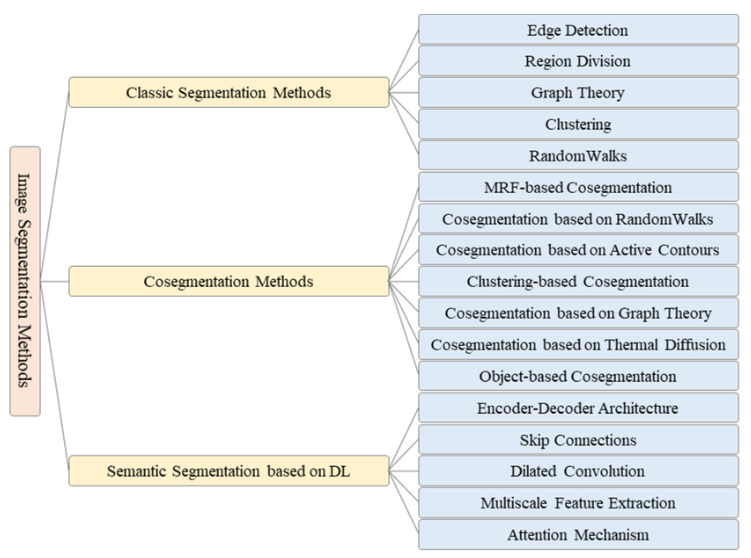
\includegraphics[scale=0.5]{imagens/metodos_segmentacao.png}
    \label{fig:segmentacao}
\end{figure}
\FloatBarrier

\section{Segmentação Baseada em Camadas}

No documento feito por \citeauthorandyear{electronics12051199} A \textbf{segmentação clássica} inclui técnicas que se concentram em características locais da imagem, como bordas e regiões como citado pelos outros autores também, mas ele aborda alguns conceitos diferentes como a \textbf{co-segmentação}, que foca na extração de objetos comuns em múltiplas imagens, considerando informações de contexto para identificar objetos similares. Por fim, a \textbf{segmentação semântica com \textit{Deep Learning}} incorpora redes neurais profundas que identificam objetos com precisão ao aprender características complexas diretamente de grandes conjuntos de dados anotados.

A segmentação baseada em camadas, conforme proposta por \citeauthorandyear{6042883}, é uma abordagem que organiza objetos em uma hierarquia de camadas, onde cada camada representa um objeto ou uma parte de objeto na imagem. Essa técnica permite que objetos sejam compostos e organizados em uma estrutura que leva em consideração tanto a aparência quanto a profundidade relativa de cada objeto na cena.

O método de \citeauthorandyear{6042883} utiliza máscaras de forma derivadas de detectores de objetos, as quais são compostas em camadas para criar uma segmentação que engloba tanto rótulos de classe quanto rótulos de instância. Com isso, a abordagem considera a organização espacial e relacional dos objetos, permitindo a detecção de elementos mesmo quando oclusos ou parcialmente visíveis, ao inferir o layout da cena com base em uma distribuição probabilística das camadas.

Cada camada é ordenada em profundidade, atribuindo objetos com maior pontuação em primeiro plano e outros objetos em segundo plano. Essa estruturação permite que o sistema identifique transições e relacionamentos entre diferentes camadas, ajudando a criar segmentações precisas, principalmente em cenários complexos onde múltiplas instâncias de objetos podem se sobrepor ou interagir de forma dinâmica. A partir dessa hierarquia, o modelo é capaz de reconciliar informações de alto nível com detalhes de baixo nível, integrando informações de cor e textura com os contornos e formatos dos objetos segmentados.

A segmentação em camadas não só melhora a precisão da rotulação de pixels, mas também possibilita uma compreensão mais profunda das interações entre objetos. Essa característica é particularmente vantajosa para a segmentação de imagens que contêm múltiplas instâncias e classes, onde a separação de camadas facilita a correta identificação de fronteiras e a resolução de ambiguidades visuais.

\section{Segmentação baseada em blocos}

Já os métodos de Segmentação de Imagem Baseados em Blocos, segundo \citeauthorandyear{ZAITOUN2015797}, podem ser categorizados em duas propriedades principais: descontinuidade e similaridade. Essas técnicas de segmentação dividem-se em várias abordagens, incluindo aquelas que se concentram em características como cor, continuidade, similaridade e bordas, permitindo a criação de subcategorias específicas de acordo com o processo de divisão aplicado.

Entre as abordagens principais, destacam-se os métodos baseados em bordas abordado por \citeauthorandyear{Mayangky_Merlina_Prasetyo_Amelia_Irsictia_Putri_2024}, que se concentram em detectar descontinuidades na intensidade da imagem para identificar transições abruptas entre diferentes objetos ou regiões. Alguns dos métodos clássicos de detecção de bordas incluem a \textbf{Detecção de Bordas de Roberts}, que utiliza operadores cruzados para calcular o gradiente espacial e é amplamente valorizada pela simplicidade e eficiência, sendo ideal para aplicações que exigem baixo custo computacional; a \textbf{Detecção de Bordas de Prewitt}, que calcula a magnitude e orientação das bordas usando uma máscara de convolução 3x3, tornando-se mais robusta do que o método de Roberts, embora ainda suscetível a ruídos; e a \textbf{Detecção de Bordas de Sobel}, que aplica uma máscara 3x3 rotacionada em 90º para suavizar ruídos enquanto calcula o gradiente das bordas, sendo amplamente utilizada devido à sua eficácia na detecção de bordas.

Com os avanços na inteligência artificial e nas técnicas de computação evolutiva, surgiram métodos de detecção de bordas mais sofisticados. Entre eles, o método \textbf{Baseado em Lógica Fuzzy} que é descrito por \citeauthorandyear{info8030104} como uma lógica que utiliza conjuntos fuzzy que permitem que cada pixel pertença a múltiplas regiões, oferecendo flexibilidade em imagens com transições suaves. Já o método \textbf{Baseado em Algoritmos Genéticos} inspira-se na teoria da evolução, utilizando processos de seleção, cruzamento e mutação para identificar as bordas de maneira eficiente, sendo particularmente útil em padrões complexos. O método \textbf{Baseado em Redes Neurais}, por sua vez, utiliza redes neurais artificiais treinadas para aprender padrões de bordas ajustando os pesos entre suas camadas, sendo altamente eficaz na detecção de bordas em cenários com variabilidade de padrões. 

A integração do big data com o avanço dos hardwares modernos permitiu que a inteligência artificial atingisse novos patamares de desempenho na segmentação de imagens. A habilidade de processar grandes volumes de dados possibilita que a IA identifique padrões e características em imagens de maneira rápida e precisa. Segundo \citeauthorandyear{carvalho_2021}, o uso de \textit{deep learning} e de técnicas de machine learning aprimora ainda mais essa precisão, tornando a segmentação detalhada e eficiente, essencial para diversas aplicações inovadoras.

\section{Segment Anything}

Inserido nesse contexto e com base no artigo criado por \cite{kirillov2023segany} o modelo Segment Anything (SAM) é um novo avanço na área de segmentação de imagens, proporcionando uma abordagem generalista que visa resolver diversos problemas de segmentação utilizando diferentes tipos de dados e prompts. Com um conjunto de dados extenso e uma arquitetura inovadora, o SAM permite a criação de máscaras de segmentação em tempo real e com capacidade de generalização para novos conjuntos de dados.

\subsection{Motivação e Contexto}

A segmentação de imagens tem sido revolucionada pelo surgimento de métodos de \textit{deep learning}, como o Segment Anything Model (SAM), que permite uma segmentação versátil e de alta escala. A segmentação de imagem visa identificar e isolar regiões ou objetos dentro de uma imagem, o que é essencial em várias aplicações de visão computacional. Métodos convencionais, entretanto, exigiam grande quantidade de dados rotulados e intensa supervisão manual. O SAM introduziu uma abordagem de zero-shot, possibilitando segmentações precisas em novos conjuntos de dados sem a necessidade de re-treinamento, utilizando prompts como caixas delimitadoras e pontos para indicar regiões de interesse \cite{ke2023segmenthighquality}.

Apesar de seu impacto, o SAM apresenta limitações ao lidar com bordas complexas e objetos finos. Para superar essas limitações, o HQ-SAM foi proposto como uma extensão de alta qualidade do SAM, incorporando um token de saída especializado e técnicas de fusão de características globais e locais para melhorar a definição das bordas e a precisão da segmentação em objetos detalhados e sobrepostos. Esses avanços garantem que o HQ-SAM preserve a flexibilidade e a generalização zero-shot do SAM original enquanto aumenta significativamente a acurácia da segmentação \cite{ke2023segmenthighquality}.

\subsection{Arquitetura do SAM}

A arquitetura do SAM é composta por três principais componentes: um codificador de imagens, um codificador de prompts e um decodificador de máscaras. O codificador de imagens gera um embedding (representação) da imagem que pode ser reutilizado para diferentes prompts. O codificador de prompts permite que o SAM aceite uma variedade de entradas, como pontos, caixas delimitadoras, e até mesmo textos para identificar as áreas de interesse na imagem. O decodificador de
máscaras, então, gera as máscaras de segmentação apropriadas a partir dessas entradas. O SAM é projetado para ser eficiente, processando prompts em tempo real.

\subsection{Conjunto de Dados SA-1B}

Para treinar o SAM, foi desenvolvido o conjunto de dados SA-1B, que contém mais de 1 bilhão de máscaras de segmentação provenientes de 11 milhões de imagens. Essas imagens são diversas, de alta resolução, e foram obtidas respeitando
questões de privacidade. Esse conjunto de dados é, até o momento, o maior já construído para a tarefa de segmentação, superando os bancos de dados existentes em termos de diversidade e volume. O SAM é capaz de gerar máscaras de
segmentação automaticamente a partir dessas imagens, tornando-se uma ferramenta poderosa para a criação de novos conjuntos de dados e modelos de visão computacional.

\subsection{Aplicações e Resultados}

O Segment Anything Model (SAM) foi amplamente testado em tarefas de segmentação, como a segmentação de objetos a partir de pontos, detecção de bordas e segmentação de objetos sobrepostos, demonstrando forte desempenho e flexibilidade. Em cenários complexos, o SANeRF-HQ aprimora o SAM para segmentação em 3D de alta qualidade, utilizando prompts e campos de densidade para garantir consistência entre múltiplas visualizações. Os resultados mostram uma melhoria significativa em relação aos métodos anteriores, mantendo generalização zero-shot e alta acurácia ao longo de diferentes conjuntos de dados \cite{liu2024sanerfhqsegmentnerfhigh}.

\subsection{Comparações com Métodos Tradicionais}

O SAM apresenta várias vantagens em relação a métodos tradicionais de segmentação, como o Crescimento de Regiões. Enquanto os métodos tradicionais exigem parâmetros e pré-processamento mais específicos para funcionar corretamente, o SAM, por meio de sua arquitetura flexível e escalável, permite segmentação em uma ampla gama de imagens com menos intervenção manual. Além
disso, sua capacidade de processar múltiplas máscaras para um único prompt o torna eficaz para cenários onde a ambiguidade está presente, como a detecção de partes de objetos sobrepostos.

\section{Trabalhos Correlatos}

Nesta seção são apresentados os trabalhos correlatos ao proposto neste trabalho

\subsection{Segmentation by grouping junctions}

A segmentação de imagens tem evoluído significativamente com a introdução de métodos baseados em aprendizado profundo.\citeauthorandyear{minaee2020imagesegmentationusingdeep} realizam uma extensa revisão sobre métodos de segmentação com redes neurais, destacando abordagens como redes totalmente convolucionais (FCN), arquiteturas encoder-decoder e redes piramidais de múltiplas escalas, que são amplamente adotadas. Estes métodos permitiram avanços consideráveis na precisão e na generalização dos modelos, especialmente para aplicações em imagens médicas e na análise de cenas complexas, onde a precisão é crucial.

\subsection{Monocular depth estimation based on deep learning: An overview}

A estimação de profundidade monocular é um problema fundamental em visão computacional. Métodos baseados em aprendizado profundo (deep learning) têm sido estudados e alcançaram resultados promissores. Existem três categorias de métodos: supervisionados, não supervisionados e semi-supervisionados. Arquiteturas de rede neural como CNNs, RNNs e GANs são utilizadas. O artigo de \cite{zhao2020monocular} apresenta uma visão geral desses métodos e discute desafios e oportunidades.